\chapter{Introdução}

Estimativas de recursos e reservas minerais demandam a construção de modelos numéricos de teores de longo prazo, que abrangem toda a extensão do depósito mineral e compreendem todo o tempo de vida da mina. Esses modelos são atualizados em intervalos de um a três anos de operação. Modelos de médio prazo podem ser construídos para planejar de um a seis meses no futuro do empreendimento. Enquanto modelos de curto prazo, são construídos com o objetivo de balizar, semanalmente ou diariamente, as decisões relativas a controle de teores e planejamento detalhado da mina.

Construir modelos numéricos de longo, médio e curto prazo para avaliação de recursos/reservas e planejamento de mina exige quatro grandes atividades \cite{rossi2013mineral}:

\begin{enumerate}
\item Coleta e gerenciamento de dados;
\item Interpretação e modelagem geológica;
\item Atribuição de teores;
\item Avaliação e gerenciamento da incerteza geológica e de teores.
\end{enumerate}

Após a coleta, gerenciamento e checagem dos dados, é necessário identificar diferentes domínios. A determinação dos domínios deve ser baseada no conhecimento geológico, i.e. zonas de oxidação, litologias, alteração ou limites estruturais e deve ser suportada por extensiva análise estatística (análise exploratória dos dados), incluindo análises variográficas. É importante que a definição dos domínios faça sentido espacial e geológico. Os domínios são, algumas vezes, baseados na combinação de duas ou mais variáveis para as quais a correlação entre os teores pode ser demonstrada. O procedimento pode ser bastante demorado, principalmente em depósitos multivariados, entretanto, as estimativas são melhoradas significativamente quando cuidadosamente limitadas por variáveis geológicas \cite{rossi2013mineral}.

A definição de diferentes domínios de estimativas, ou zonas estacionárias no interior do depósito, é necessária porque a inferência geoestatística, geralmente, o método de escolha para a construção dos modelos numéricos de teores, exige decisão de estacionariedade \cite{mclennanstationarity}. Isto é, os teores em cada domínio estacionário pertencem a populações estatísticas distintas, são caracterizados através de modelos de distribuição e de covariância específicos e devem ser modelados como funções aleatórias estacionárias diferentes. \cite{journel1978mining}. 

Uma função aleatória estacionária é uma representação probabilística de uma propriedade petrofísica com valor esperado e covariância constantes independente da localização \cite{mclennanstationarity}. Estacionariedade, definida por \citeonline{matheron1962traite}, é uma propriedade do modelo de função aleatória, não é uma característica intrínseca da variável. É uma decisão tomada pelo geomodelador e necessária para a inferência.

Os domínios estacionários não devem ser muito pequenos, dessa forma não existirão dados suficientes para descrição e inferência estatística confiável, e nem muito grandes, já que os dados, provavelmente, poderiam ser subdivididos em grupos geologicamente mais homogêneos. A definição adequada dos domínios estacionários é uma etapa importante na avaliação de recursos/reservas, a mistura de populações produz estimativas sub ótimas que superestimam ou subestimam teores e tonelagens. Além disso, nenhuma técnica geoestatística pode compensar uma definição de estacionariedade inadequada \cite{rossi2013mineral}.

Uma vez que os domínios estacionários tenham sido definidos, um modelo tridimensional que defina os limites de cada função aleatória estacionária deve ser construído: o modelo geológico. É necessário identificar a "jurisdição espacial" de cada função aleatória estacionária. Inevitavelmente, existe incerteza associada à localização dos limites, e essa incerteza geológica deve ser quantificada \cite{mclennanstationarity}. A etapa de Interpretação e modelagem geológica compreende a definição dos domínios estacionários e a criação do modelo geológico tridimensional que forma o alicerce para todo o trabalho de estimativa subsequente. Muitas vezes, o modelo geológico é o fator de maior importância na estimativas das tonelagens mineralizadas \cite{rossi2013mineral}.

A abordagem tradicional para a criação de modelos geológicos tridimensionais é através da triangulação de polilinhas \footnote{Em computação gráfica: uma linha composta por vários segmentos, usada para compor imagens na tela \cite{oxfordonlinedictionary}.} (\textit{strings}) gerando sólidos que representam os corpos minerais. As polilinhas são digitalizadas manualmente em seções deslocadas, a partir dos dados de sondagem e conhecimento geológico prévio, por um geomodelador. As seções são unidas por linhas guias, que demarcam a conectividade entre as seções digitalizadas para triangulação adequada dos sólidos. Esse procedimento é referido como modelagem geológica explícita, já que a os limites entre os diferentes domínios são definidos explicitamente por coordenadas (x,y,z) que posicionam a "colcha de retalhos" de triângulos \cite{mclennan2006boundsim,cowan2003practical}. A \autoref{explicitmodeling} ilustra a metodologia explícita para um típico depósito de veio.

\begin{figure}[H]
	\caption{\label{explicitmodeling}Ilustração esquematizando a modelagem geológica explícita usando polilinhas e linhas guias.}
	\begin{center}
		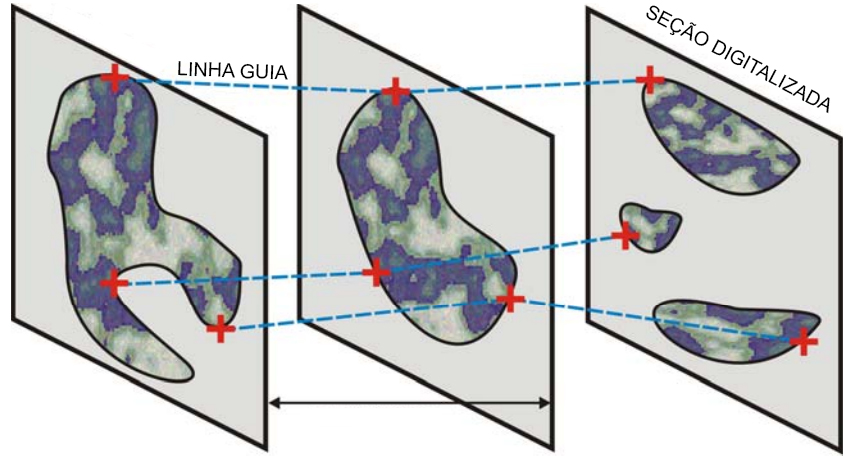
\includegraphics[width=0.6\textwidth]{capitulo_1/explicitmodeling}
	\end{center}
	\legend{Modificado de \citeonline{mclennan2006boundsim}}
\end{figure}

De acordo com \citeonline{mclennan2006boundsim}, embora a metodologia seja direta e simples, principais motivos da sua ampla implementação na prática, e que \textit{softwares} modernos de mineração forneçam ferramentas computais para visualizar os dados de sondagem e agilizar o processo de digitalização \cite{silvaenhancedgeomodeling}, existem uma série de limitações e desvantagens. O processo é tedioso e demorado, digitalizar manualmente as polilinhas e uni-las por linhas guia, exige muito tempo de um profissional experiente. Em depósitos de alta complexidade, não é raro o geomodelador trabalhar até três meses no modelo geológico explícito. A geometria dos corpos geológicos muitas vezes precisa ser simplificadas para que o modelo seja concebido em tempo hábil. Por esse motivo, para a maioria das minas, apenas um modelo é construído e mantido, raramente há oportunidade de modelar interpretações geológicas alternativas e comparar estimativas de recursos baseadas em diferentes modelos \cite{cowan2003practical}.

Os modelos criados explicitamente são subjetivos e não replicáveis. O volume mineralizado é essencialmente composto por por uma série de pequenas decisões subjetivas, já que cada ponto da polilinha em cada seção é escolhido por um geomodelador. Inevitavelmente, a "assinatura" do profissional é impressa nos limites dos domínios geológicos. Geomodeladores diferentes criam modelos diferentes a partir do mesmo banco de dados. Ademais, modelos explícitos são inflexíveis, é laborioso e demorado atualizar modelos explícitos a medida que novos dados são obtidos já que uma nova digitalização manual é necessária.

Em virtude da onerosidade em construir múltiplos modelos geológicos explícitos, é custoso avaliar a incerteza na localização dos limites dos diferentes domínios entre os dados amostrais, como mostrado na ilustração esquemática na \autoref{incerteza_limites}. Além da tediosa redigitalização manual de polilinhas e retriangulação, não existe forma direta de incorporar múltiplas realizações possíveis para a localização dos limites que representam a incerteza associada.

\begin{figure}[H]
	\caption{\label{incerteza_limites}Ilustração esquemática destacando a incerteza na localização do limite entre os domínios azul e vermelho, entre os dados amostrais.}
	\begin{center}
		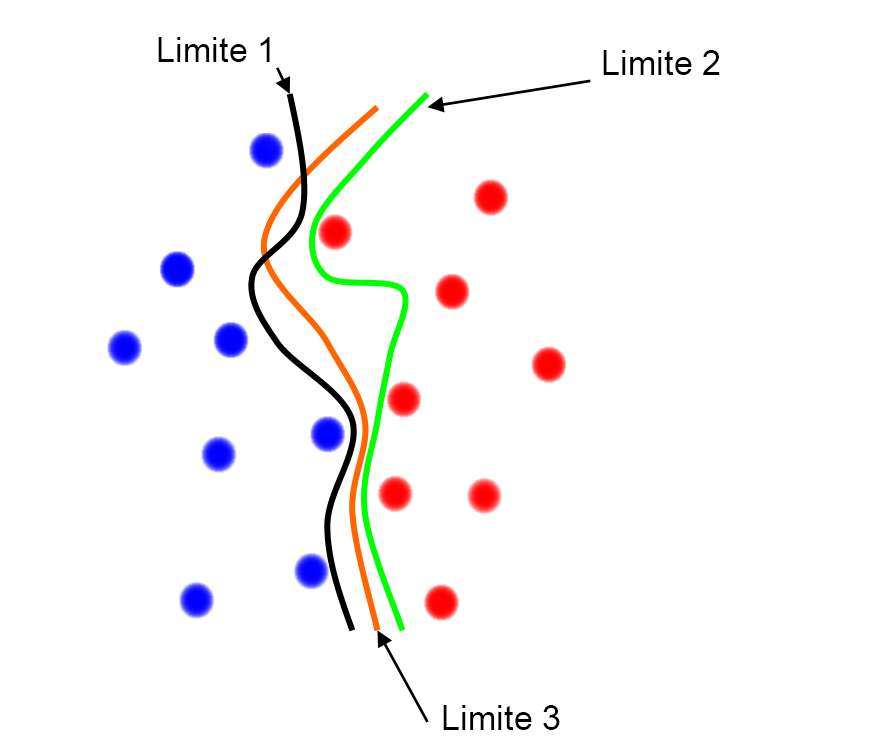
\includegraphics[width=0.6\textwidth]{capitulo_1/incerteza_limites}
	\end{center}
	\legend{Modificado de \citeonline{caceres2011stochastic}}
\end{figure}

Em muitos casos, a incerteza do modelo geológico pode ser uma fonte de incerteza crucial. Em depósitos de veio de ouro, por exemplo, o volume mineralizado é um indicador econômico vital para o gerenciamento do projeto. Ignorar a incerteza volumétrica, considerando apenas um único modelo geológico explícito, pode ser ser devastador para o empreendimento. A incerteza associada ao modelo geológico deve ser avaliada.

Embora a metodologia explícita seja demorada, laboriosa, subjetiva, não replicável, inflexível e incapaz de avaliar incertezas, o limites entre domínios resultantes, geralmente, são realistas. Realismo geológico é um dos principais objetivos da modelagem e pode ser diretamente controlado durante o processo de digitalização. 

Dadas as desvantagens do método explícito de modelagem geológica, pesquisas vêm sendo realizadas com o objetivo de automatizar, ou pelo menos, semi automatizar a modelagem. Métodos matemáticos menos sofisticados, como o vizinho mais próximo podem ser utilizados na criação automática de modelos geológicos determinísticos.  Métodos geoestatísticos também têm aplicação, a krigagem dos indicadores, \cite{journel1982indicator} consiste na geração de uma distribuição acumulada de probabilidades a partir da transformação não linear dos dados. Para variáveis categóricas, é possível estimar diretamente a probabilidade de cada local não amostrado pertencer à cada uma das diferentes litologias do depósito mineral.

A necessidade de avaliação da incerteza associada ao modelo geológico impulsionou o desenvolvimento de métodos estocásticos baseados em múltiplas realizações equiprováveis de um atributo. A partir da análise conjunta das realizações é possível avaliar a incerteza. 

São metodologias estabelecidas da geoestatística clássica, baseada no variograma: a simulação sequencial dos indicadores \cite{goovaerts1997geostatistics}, que compartilha do mesmo princípio da krigagem dos indicadores. A simulação gaussiana truncada \cite{matheron1987conditional}, que tem como ideia central gerar múltiplas realizações de uma variável aleatória gaussiana contínua e truncá-las em uma série de limites pré definidos, indicando as diferentes litologias. A simulação plurigaussiana truncada, \cite{galli1994pros} que é uma extensão da simulação gaussiana truncada, baseada na truncagem de duas funções aleatórias gaussianas que podem ou não ser correlacionadas.

Outras metodologias não baseadas em variograma foram desenvolvidas: a simulação geoestatística multiponto \cite{strebellesimulationscomplexgeology}, tem o mesmo formalismo das simulações sequenciais baseadas em variograma, com a diferença que a distribuição local de probabilidade é encontrada a partir da amostragem de uma imagem de treinamento com um modelo multi ponto \cite{pyrcz2014geostatistical}. Do mesmo modo, a simulação baseada em objetos \cite{alabert1992stochastic, bratvold1995storm, holden1998modeling}, metodologia que produz modelos atrativos (visualmente limpos) que honram a geometria idealizada interpretada a partir de afloramentos ou dados de sísmica. Quando geometrias específicas do depósito ou reservatório são identificadas de forma correta, parametrizadas e têm significância para a função de transferência, podem ser integradas diretamente no modelo pelos métodos baseados em objetos \cite{pyrcz2005stochastic}. 

Uma outra família de métodos, ditos métodos implícitos, compreendem técnicas importadas da computação gráfica. O uso da modelagem implícita foi introduzida no campo da computação gráfica para a geração de objetos de diferentes geometrias e complexidades por  \citeonline{bloomenthal1997introduction}. A ideia geral é usar uma função implícita para demarcar regiões de diferentes formas e extensões no espaço. \citeonline{cowan2002rapid,cowan2003practical} popularizou a modelagem implícita no contexto geológico, baseado no trabalho de \citeonline{savchenko} que modela objetos tridimensionais a partir de dados esparsos interpolando uma função volume (\autoref{busto}).

\begin{figure}[H]
	\caption{\label{busto}Busto reconstruído a partir de pontos esparsos.} 
	\begin{center}
		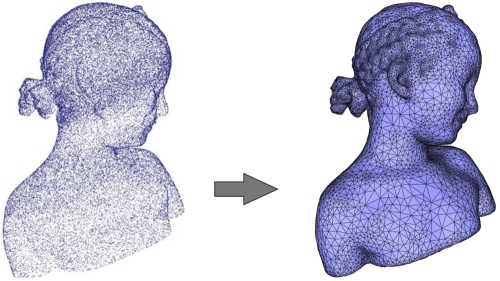
\includegraphics[width=0.6\textwidth]{capitulo_1/busto}
	\end{center}
	\legend{Fonte: \citeonline{poisson_recon}}
\end{figure}

Modelos geológicos implícitos são criados a partir de dados esparsos, geralmente, dados categóricos (\autoref{imp_mod} (a)). Os pontos amostrais podem ser usados para derivar uma função implícita que fornece uma representação matemática contínua de um atributo através de um volume, um campo escalar ou modelo implícito (\autoref{imp_mod} (b)). Modelos implícitos contém um número infinito de isosuperfícies, para visualizar o modelo geológico uma isosuperfície específica deve ser extraída do modelo e mostrada no espaço tridimensional (geralmente a isosuperfície zero), $f(x,y,z)=s$, onde $s$ é o valor de interesse no campo escalar (\autoref{imp_mod} (c)). A localização dessa superfície é conhecida implicitamente como função da localização no domínio \cite{martin2017implicitmodeling}. 

\begin{figure}[H]
	\caption{\label{imp_mod}Ilustração esquemática da modelagem geológica implícita.}
	\begin{center}
		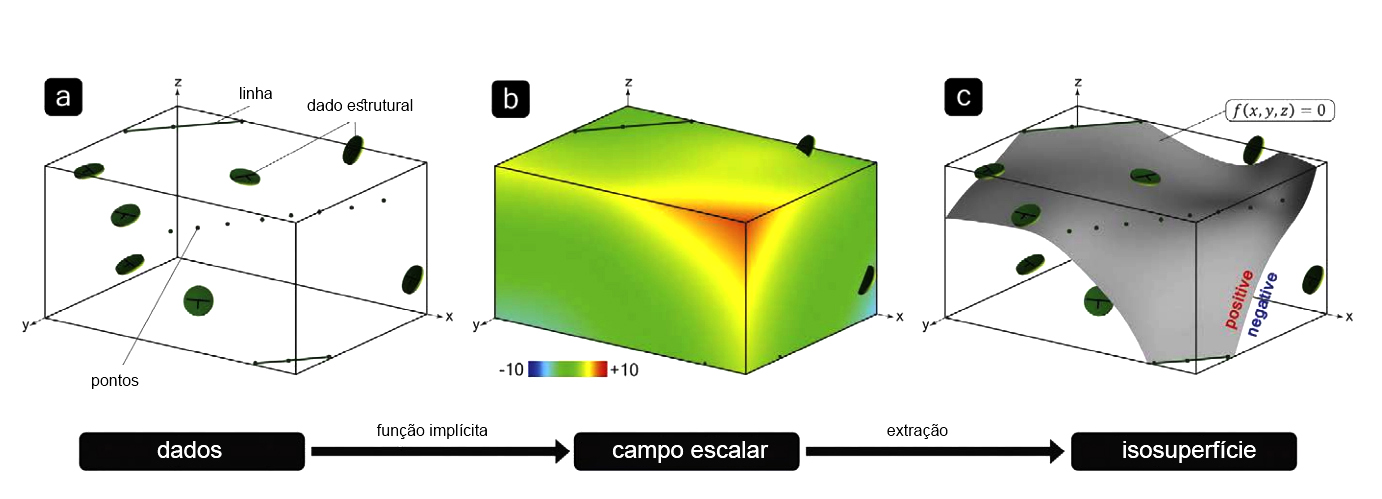
\includegraphics[width=\textwidth]{capitulo_1/implicit_modelig_pt_1}
	\end{center}
	\legend{Modificado de \cite{aillerespresentation}}
\end{figure}

Diferentes tipos de dados amostras podem ser usados para derivar diferentes funções volume na modelagem implícita. \citeonline{mallet2004space} propõe uma função volumétrica cronológica, levando em consideração a posição estratigráfica das diferentes unidades geológicas, enquanto \citeonline{lajaunie1997foliation} usam co-krigagem de incrementos em um campo potencial, omitindo a função volume. A função volume mais comumente utilizada é a função distância assinalada \cite{osherlevelsetmethods}, a aplicação dessa metodologia é encontrada por toda a literatura de interpolação de dados esparsos, uma das aplicações é a reconstrução de superfícies a partir de escaneamento (\autoref{busto}). Na modelagem geológica a metodologia é competente em capturar a geometria e extensão de corpos geológicos e tem sido aplicada com sucesso há mais de 10 anos na exploração mineral tendo ganhado espaço em softwares comerciais como o \textit{Leapfrog \textsuperscript{\textregistered}}. Para bancos de dados pontuais, que representam a posição espacial de diferentes litologias no espaço, o uso das funções distância assinaladas torna os processos de interpretação, cálculo, modelagem, modificação do modelo de acordo com a interpretação dos geomodeladores e avaliação da incerteza diretos e rápidos. Além disso, informações a respeito da orientação das unidades geológicas (dados estruturais) pode ser imputada como restrição na criação do modelo geológico \cite{martin2017implicitmodeling}.